\chapter{Grundlagen \& Stand der Technik}
\label{kap:Grundlagen}
\minitoc\pagebreak


\section{Visualisierung von Daten}
\label{sec:visual}
Ein großer Aspekt dieser Arbeit ist das Darstellen und Visualisieren von gemessenen oder generierten Daten.
Dies beschreibt den Vorgang vorhandene Daten, die in heterogenen Formaten und Typen vorliegen, in eine visuelle, grafische Form umzuwandeln, sodass sie für den Menschen leichter wahrzunehmen und lesbar sind.
Mit einem einzigen Blick können mehrere Tausend Daten(-punkte) auf einmal verarbeitet werden.
Dabei kommt die Visualisierung zuerst als Sinnes-Reiz beim Betrachter an, daraufhin wird sie identifiziert, wahrgenommen und interpretiert \cite{Goldstein.2015, FischerStabel.2018}.
Für die gleiche Datenmenge bräuchte ein Mensch unvergleichbar mehr Zeit, um die selbige Interpretation der Daten zu erhalten.

Diese Möglichkeit, der schnellen und effizienten Interpretation für die vorliegenden Daten dieser Arbeit  bereitzustellen, ist eine der Zielstellungen.
Hierfür müssen vorab diverse Grundlagen gelegt werden, damit diese bei der späteren \fullref{kap:anforderungsanalyse}, \fullref{kap:konzept} und \fullref{kap:umsetzung} stets beachtet werden.

\subsection{Definitionen}
Zunächst werden grundlegende Begriffe wie Daten, Datenanalyse oder Visualisierung definiert, damit eine einheitliche Basis geschaffen wird.
\subsubsection{Daten}
Daten sind gemäß \cite{Dudenredaktion.2015}:
\begin{quote}
\glqq durch Beobachtungen, Messungen, statistische Erhebungen gewonnene [Zahlen]werte, [...] Angaben, formulierbare Befunde. \\
EDV: elektronisch gespeicherte Zeichen, Angaben, Informationen\grqq{}
\end{quote}

Demnach gibt es heterogene Daten, welche in Form von Zahlen, Buchstaben, Texten vorliegen können.
In Anblick auf die vorliegenden Daten dieser Arbeit gibt es beispielsweise gemessene Vitaldaten von Patienten wie Herz- \& Atemfrequenz oder die Sauerstoffsättigung.
Weiter sind auch vereinzelt Angaben zu dem Patienten, wie das Alter, oder generelle Informationen wie der Tag und die Uhrzeit eines Einsatzes als Daten gespeichert.
 
\subsubsection{Datenanalyse}
Daten können analysiert werden.
Dabei bezeichnet die Analyse die strukturierte Untersuchung von Elementen, welche zunächst aufgeteilt und geordnet werden, damit anschließend eine Auswertung betrieben werden kann.
Dabei kann laut Fischer \cite{Fischer.2014} grundlegend zwischen zwei Formen der Analyse unterschieden werden: konfirmativ und explorativ.
\begin{description}
\item[konfirmative Analyse] bezeichnet die Überprüfung von bestehenden Hypothesen.
Dabei werden bekannte Methoden angewandt, um die jeweilige Hypothese zu bestätigen oder zu widerlegen.
\item[explorative Analyse] ist gekennzeichnet durch das Fehlen von gestellten Hypothesen.
Hierbei wird nach neuen Erkenntnissen oder Fragestellungen gesucht, welche durch Trends, Muster oder Beziehungen entdeckt werden.
\end{description}

Da bei dieser Arbeit das zu untersuchende Element der Analyse stets Daten sind, handelt es sich in diesem Kontext immer um \glqq Datenanalysen\grqq{} \cite{Schumann.2000}.
Es kommen hier sowohl explorative als auch konfirmative Datenanalysen zum Einsatz, da es bereits bestehende Hypothesen in Form von Fragestellungen der Nutzer gibt.
Andererseits gibt es auch vermeintlich viele, bisher unbekannte, Zusammenhänge, welche durch die Interaktion der Anwender mit den Visualisierungen zum Vorschein kommen können.


\subsubsection{Visualisierung}
Eine Visualisierung ist nach McCormick \cite{Mccormick.1987} das transformation von Information in geometrische Repräsentation von graphischen Objekten.
Dies erleichtert dem Menschen die Aufnahme von Informationen, insbesondere aber das erkennen von Zusammenhängen und Strukturen innerhalb der Daten.
Die Subjektivität der Individuen ermöglicht keine einwandfreie Garantie des Informationsflusses zum jeweiligen Anwender. %\cite{Fischer.2014}. 
Auch kann unterschieden werden, ob eine Visualisierung unterstützend zu einer Niederschrift beiträgt, oder sie als Haupt-Informationsquelle die tragende Figur ist \cite{Bassler.2010}.
Im Zuge dieser Arbeit wird letzteres das Mittel der Wahl sein.

Nach \cite{Card.2007} kann die Datenvisualisierung als besondere Form einer Visualisierung abgegrenzt werden.
Dabei gibt es fünf Eigenschaften, die eine solche spezielle Form klassifizieren:
\begin{itemize}
\item Computergestützte Anzeige 
\item Der Nutzer kann interaktiv Auswahlen treffen oder Filter bestimmen, um die anzuzeigenden Daten einzuschränken
\item Die Eigenschaften der Daten werden in visuellen Elementen wie Form, Farbe oder Größe unterschiedlich dargestellt
\item Abstrakte Daten können dargestellt werden, welche keiner physischen Form zugrunde liegen
\item Die Fähigkeiten des Menschen in Bezug auf die Wahrnehmung wird berücksichtigt 
\end{itemize}

Demzufolge wird im Kontext dieser Arbeit der Begriff Datenvisualisierung und Visualisierung synonym verwendet, die die entsprechenden Eigenschaften auf die hier erarbeiteten Visualisierungen zutreffen.
\todotext{konfirmativ und explorativ visualis (fischer s.26?}

%WordCloud
Es gibt nach \cite{Schumann.2000} einen \glqq Visualisierungsprozess\grqq{}, welcher den Weg von Rohdaten bis zum Bild abstrahieren soll.

\bild
{visualprozess}
{8cm}
{Der Prozess einer Visualisierung von den Rohdaten zum fertig generierten Bild. Bildquelle \cite[S.50]{FischerStabel.2018} (verändert)}
{Der Prozess einer Visualisierung}

Dieser Prozess ist in Abbildung \ref{fig:visualprozess} erkennbar.
Nachfolgend werden die einzelnen Phasen kurz erläutert:
\begin{description}
\item[Rohdaten] In der ersten Phase muss eine oder mehrere Quellen der Daten festgelegt werden. 
Anschließend wird grob gesichtet und so eine Datenbasis gelegt.
\item[Filtering] Anschließend werden die Rohdaten aufbereitet, wobei beispielsweise eine Bereinigung, Interpolation oder Neuberechnung von Daten vorgenommen werden
\item[Mapping] Daraufhin kommt nach \cite{FischerStabel.2018} das Hauptproblem der Visualisierung: Die Auswahl einer geeignet Darstellungsform passend zu den Daten. 
Dabei gibt es diverse Möglichkeiten, welche Darstellungsform mit welchen Attributen (Größe, Farbe, Form) umgesetzt wird. 
\item[Rendering] Als Letztes werden die aufbereiteten Daten mit der gewählten Darstellungsform als Bild oder interaktive Visualisierung erzeugt.
Dies geschieht heutzutage häufig über sogenannte \gls{BI}-Werkzeuge wie Qlik (siehe \ref{qlik})
\end{description}




\subsection{Gestaltungsgrundsätze}
\label{sub:grundsätze}
In der Wahrnehmungspsychologie gibt es diverse Erkenntnisse, wie das menschliche Gehirn unterschiedliche Muster und Strukturen erkennt.
Dabei sind diese Fähigkeiten größtenteils evolutionär geprägt, da es für den Menschen schon immer wichtig war, schnell Entscheidungen zu treffen, oder komplexe neue Aufgabestellungen zu lösen.
Dabei greift das Gehirn auf zuvor erlernten oder erlebten Ereignissen zurück, um neue Aufgaben klassifizieren zu können.

Heutzutage finden sich die Auswirkungen dieser Prägungen in dem Alltag jedes Menschen wieder.
Dabei ist die Form der Wahrnehmung nie objektiv, sondern stets subjektiv, da diese Fähigkeit der Mustererkennung auf Basis von Erfahrungen aufbaut, welche bei jedem Menschen im Laufe des Lebens unterschiedlich sind.
Dies ist eine wichtige und essentielle Erkenntnis, da hierbei die Interpretation von Datenvisualisierungen divergieren kann \cite{Fischer.2014}.

Dennoch gibt es diverse Grundregeln, welche sich im Laufe der Jahrtausende bei den Menschen durchgesetzt haben. Diese wurden zuerst von Wertheim in seiner Forschung \glqq Lehre von der Gestaltung\grqq{} schriftlich festgehalten \cite{Wertheimer.2017}.
Nach und nach wurden diese von mehreren Psychologen oder Designern unter den \glqq Gestaltungs-Gesetzen\grqq{} oder -Prinzipien aufgefasst undabgewandelt, wodurch sie sich indes unterscheiden.
Nachfolgend werden fünf, für Diagramme und Visualisierungen relevante Gesetze nach \cite[5.2]{Heber.2018} \& \cite{Ware.2009} näher betrachtet. 
Hierbei sind vor allem bei Visualisierungen mit Zahlen, wie sie in dieser Arbeit größtenteils vorliegen werden, die ersten beiden Gesetze von sehr hoher Relevanz.

\subsubsection{Das Gesetz der Nähe}
\begin{figure}[ht]
\begin{subfigure}{.5\linewidth}
  \centering
  % include first image
  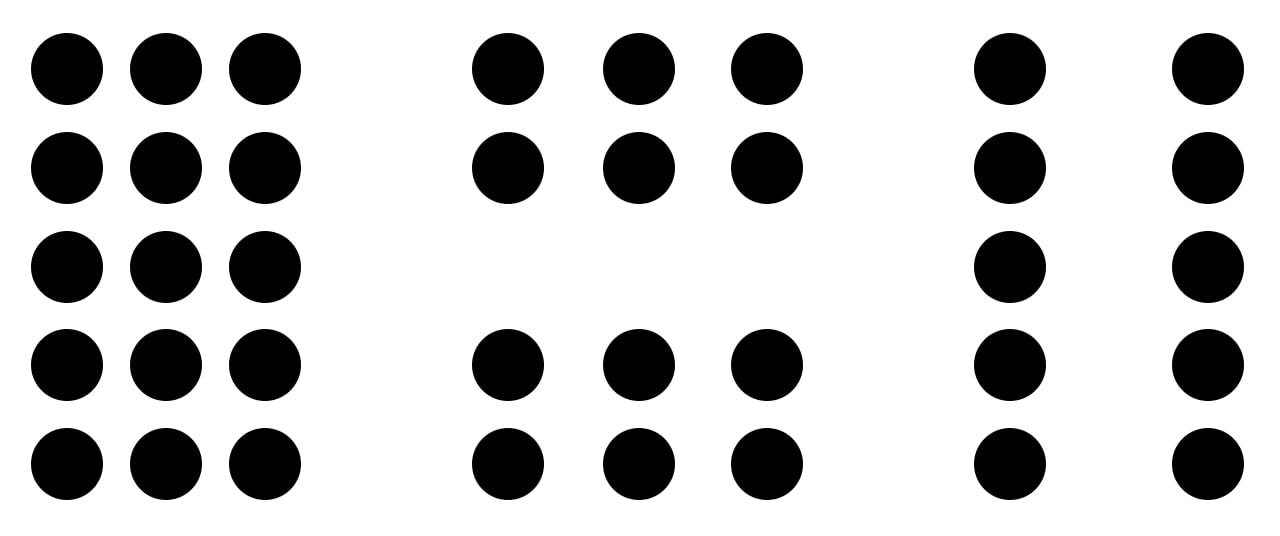
\includegraphics[width=.95\linewidth]{img/gNaehe}  
  \caption{Schematische Darstellung zur Nähe}
  \label{fig:naeheSchema}
\end{subfigure}
\begin{subfigure}{.5\linewidth}
  \centering
  % include second image
  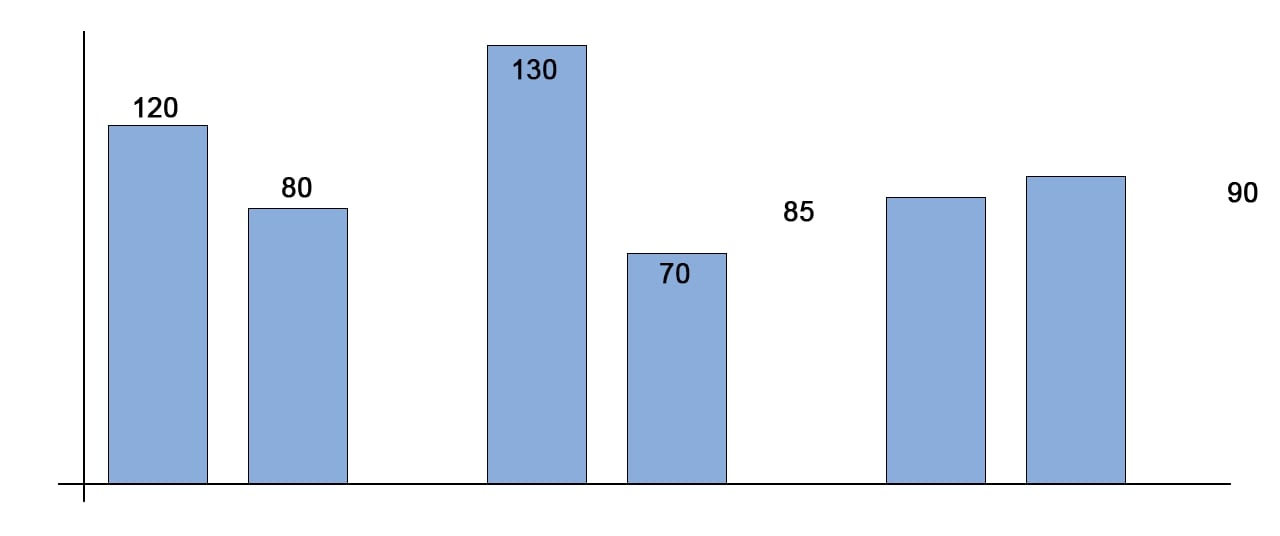
\includegraphics[width=.95\linewidth]{img/gNaeheDia}  
  \caption{Beispiel an einem Balkendiagramm mit zwei positiven und einem negativen (rechts) Beispiel}
  \label{fig:naeheDia}
\end{subfigure}
\caption[Gesetz der Nähe]{Eigene Darstellung des Gesetzes der Nähe. Links schematisch und rechts an einem Balkendiagramm dargestellt}
\label{fig:naehe}
\end{figure}
%\bild
%{gNaehe}
%{8cm}
%{Beispiel des Gesetzes der Nähe. Eigene Darstellung}
%{Gesetz der Nähe}

Das Gesetz der Nähe besagt, dass Elemente, die nahe beieinander liegen, als eine Einheit wahrgenommen werden.
Dieser Effekt ist in Abbildung \ref{fig:naehe} veranschaulicht.
Für Visualisierungen und insbesondere Diagramme bedeutet dies, dass sich beispielsweise die Zahlen immer in der Nähe des entsprechenden Elements befinden sollten.

In \ref{fig:naeheDia} ist dieser Effekt deutlich zu erkennen. 
Zum einen werden immer zwei Balken aufgrund der Distanz als Zusammengehörig wahrgenommen, zum anderen sind die Zahlen bei den ersten vier Balken gut zuzuordnen.
Bei den letzten zwei Balken sind die Zahlen zu weit entfernt und können den jeweiligen Betrachter verwirren.


\subsubsection{Das Gesetz der Ähnlichkeit}
\label{subsub:ähnlich}
\begin{figure}[ht]
\begin{subfigure}{.5\linewidth}
  \centering
  % include first image
  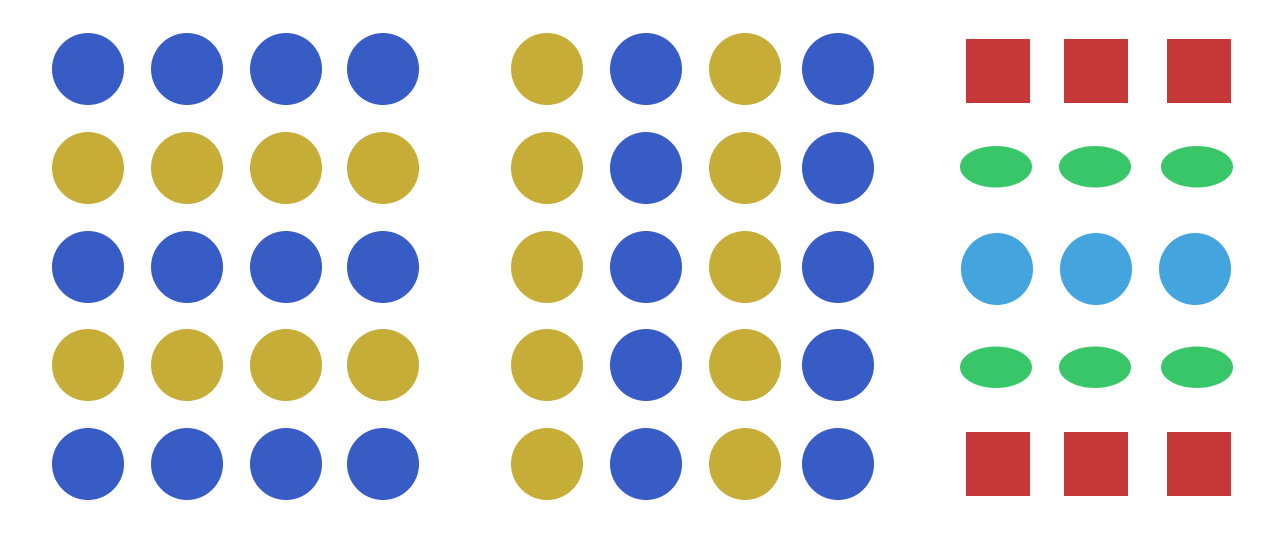
\includegraphics[width=.95\linewidth]{img/gAehnlich}  
  \caption{Schematische Darstellung zur Ähnlichkeit}
  \label{fig:aehnlichSchema}
\end{subfigure}
\begin{subfigure}{.5\linewidth}
  \centering
  % include second image
  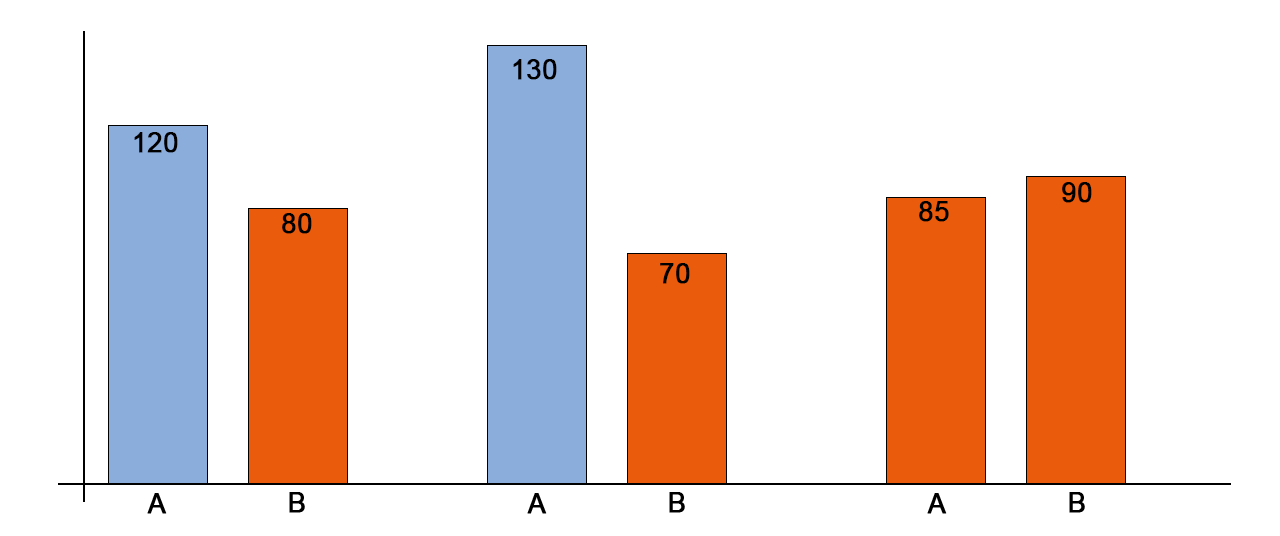
\includegraphics[width=.95\linewidth]{img/gAehnlichDia}  
  \caption{Beispiel an einem Balkendiagramm mit zwei positiven und einem negativen (rechts) Beispiel}
  \label{fig:aehnlichDia}
\end{subfigure}
\caption[Gesetz der Ähnlichkeit]{Eigene Darstellung des Gesetzes der Ähnlichkeit. Links schematisch und rechts an einem Balkendiagramm dargestellt}
\label{fig:aehnlich}
\end{figure}

Ebenfalls als eine Gruppe werden Elemente wahrgenommen, die ähnlich oder gleich aussehen.
Dabei spielen unterschiedliche Attribute wie Größe, Form oder Farbe eine Rolle.
Hier gilt, je mehr Ähnlichkeit die Elemente besitzen, desto stärker wirken sie als Einheit.

An einem Balkendiagramm ist dieses Gesetz in \ref{fig:aehnlichDia} dargestellt.
Die blauen und orangefarbenen Balken werden als Teile einer Gruppe wahrgenommen.
Die letzten beiden Balken verdeutlichen wieder ein Negativ-Beispiel: Hier werden die Balken fälschlicherweise einer Gruppe zugeordnet, obwohl sie zu zwei unterschiedlichen Gruppen gehören.
Hier wirkt außerdem das Gesetz der Nähe.


\subsubsection{Das Gesetz der Geschlossenheit}
\bild
{gGeschlossenheit}
{8cm}
{Beispiel des Gesetzes der Geschlossenheit. Eigene Darstellung}
{Gesetz der Geschlossenheit}

Das Gesetz der Geschlossenheit besagt, dass Strukturen und Formen notorisch vervollständigt werden.
Außerdem werden die vervollständigten Formen als eine zusammengehörige Gruppe wahrgenommen.

\subsubsection{Das Gesetz der Erfahrung}
\begin{figure}[ht]
\begin{subfigure}{.5\linewidth}
  \centering
  % include first image
  
\includegraphics[width=.95\linewidth]{img/gErfahrung}  
  \caption{Vervollständigung des Wortes \glqq Erfahrung\grqq}
  \label{fig:erfahrung1}
\end{subfigure}
\begin{subfigure}{.5\linewidth}
  \centering
  % include second image
  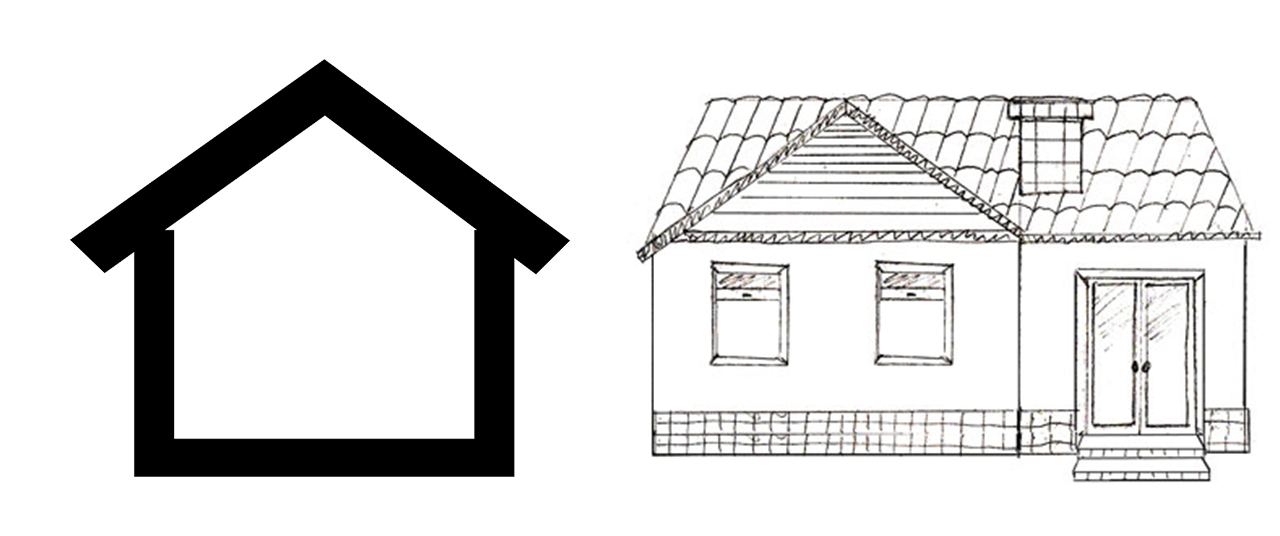
\includegraphics[width=.95\linewidth]{img/gErfahrung2}  
  \caption{Ein minimalistisches (links) und ein detailliertes Haus. Beide sind sofort zu erkennen}
  \label{fig:erfahrung2}
\end{subfigure}
\caption[Gesetz der Erfahrung]{Eigene Darstellung des Gesetzes der Erfahrung}
\label{fig:erfahrung}
\end{figure}
Das Gesetz der Erfahrung, oftmals auch der Einfachheit oder guten Gestalt genannt, bewirkt, dass unbekannte Objekte stets mit bereits bekannten Objekten abstrahiert werden.
Auch können verdeckte Texte wie in \ref{fig:erfahrung1} trotz fehlender teile gelesen werden.
Doch wenn zu viel Information verdeckt ist, ist auch keine Abstraktion auf bekannte Objekte möglich.

Bei \ref{fig:erfahrung2} wird deutlich, dass mit minimalen Informationen das Objekt klar wird.
Es sind keine Fenster, Türen, Schornstein oder anderes notwendig, damit das linke Objekt als Haus erkannt wird.

%Einfachheit
%der guten Gestalt}
\subsubsection{Das Gesetz der guten Fortsetzung}
\begin{figure}[ht]
\begin{subfigure}{.5\linewidth}
  \centering
  % include first image
  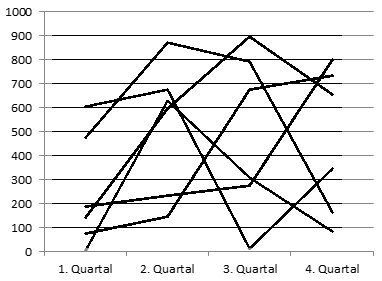
\includegraphics[width=.95\linewidth]{img/gFort}  
  \caption{Ein Liniendiagramm mit vielen schwarzen Linien}
  \label{fig:fort1}
\end{subfigure}
\begin{subfigure}{.5\linewidth}
  \centering
  % include second image
  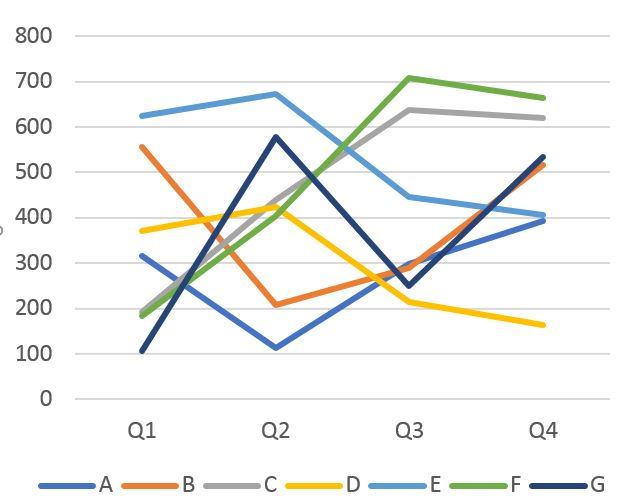
\includegraphics[width=.95\linewidth]{img/gFortC}  
  \caption{Verbesserte Lesbarkeit durch zusätzliches berücksichtigen des Gesetztes der Ähnlichkeit}
  \label{fig:fort2}
\end{subfigure}
\caption[Gesetz der Fortsetzung]{Darstellung des Gesetzes der guten Fortsetzung}
\label{fig:erfahrung}
\end{figure}

Durch das Gesetz der guten oder stetigen Fortsetzung nehmen Menschen beispielsweise kreuzende Formen so wahr, wie sie für uns am einfachsten fortgesetzt werden.
Dies ist insbesondere bei Liniendiagrammen der Fall.

In Abbildung \ref{fig:fort1} sind trotz der vielen gleichfarbigen Linien die Verläufe der einzelnen Kurven dank dieses Prinzips gut erkennbar.
Um jedoch in späteren Anwendungen die Nutzerfreundlichkeit zu erhöhen und Komplexität zu mindern, kann in einem solchen Fall das Gesetz der Ähnlichkeit (siehe \ref{subsub:ähnlich}) zusätzlich angewandt werden.
Die bessere Lesbarkeit ist in \ref{fig:fort2} zu erkennen.

\subsection{Statistische Auswertungen}
\todotext{Bild vergleich Tabelle Diagramm! (bsp fischer 4.3)}
%\subsubsection{Diagramme}
\subsection{Multidimensionale Daten darstellen}

\section{Begriffe zum Thema Data Analytics}
\subsection{Übersicht der Zusammenhänge}
\subsection{Big Data}
\subsection{Business Intelligence}
\subsection{Data Warehousing}
\subsection{Dashboards}

\section{Daten und deren Verarbeitung in der Notfallmedizin} % Rettungsdienst  
\subsection{Business Intelligence in der Notfallmedizin}
\subsection{Big Data in der Notfallmedizin}

Big Data im Gesundheitswesen\\

%Noch umschreiben! Fast 100% aus Buch
3A: Aggregation, Analyse, Auswertung
4V: Volume, Varierty, Velocity \& !med wichtig Veracity! 
Grundsätzlich nur 3V, aber Veracity ist im GEsundheitsweesen von besonderer Bedeutung. 
Volume Viele Daten: Statista DAtenvolumen.
Variety: Häufig unstrukturiert, Papier, Memo, Blog, Freteixt; Im GW besonder Rezepte, Arztmemos, Arztbriefe, Emails
Velocity: Geschwindigkeit auch wichig, besonders auch in GW, zb. weitere Befunde/ANalysen während initialer Diagnose oder erste Behandlung...
Veracity: DAten sind per se nicht gut/sclhect, qualitativ hochwertig oder mangelhaft. Daten sind neutral, wenn auch komplex sozial und technologisch Ref Gitelmann 2ff.Entscheidend ist die richtige Fragstellung im Kontext und Algorithmus. Qualitativ hochwertige Bearbeitung der Daten! \\

eHealth <-> Big Data (S.37f)
eHealth beschreibt Interface, welches mittels App, online-Plattform,... gesundheitsbezogene Dienstleistungen zur verfügung stellt, Menschen miteineander verbindet eoder technoglogische Erkenntnisse für Menschen sichtbart macht. 
- ehealth Endgeräteübergreifend, mHealth nur mobile, vHealth VR, aHealth Augemnted
- eHealth bietet Basis für Big Data, Big Data bietet Basis für eHealth, ...; nicht alles was ehealth ist, ist big data and vice versa; Trennung notwendig! picture\\

Datenquellen (relevanten Auszug davon hervorheben)(S.43f); 

\begin{table}
\centering
\caption{My caption}
\label{my-label}
\begin{tabular}{|l|l|} 
\hline
\textbf{Kategorie der Datenquelle}  & \textbf{Ausgewählte Datenquellen}                                                \\ 
\hline
Medizinische Daten                  & \begin{tabular}[c]{@{}l@{}}Vitalparameter\\ Länge des Aufenthalts \end{tabular}  \\ 
\hline
Versicherungsdaten                  & \begin{tabular}[c]{@{}l@{}}Alter\\ Name \end{tabular}                            \\ 
\hline
Öffentliche Gesundheitsdaten        & \begin{tabular}[c]{@{}l@{}}Ämter\\Gemeinden\\...\end{tabular}                    \\ 
\hline
Forschungsdaten                     & \begin{tabular}[c]{@{}l@{}}Studien\\Biobanken\end{tabular}                       \\ 
\hline
Individ. Daten                      & \begin{tabular}[c]{@{}l@{}}Ernährung\\Wellness\end{tabular}                      \\ 
\hline
Pharmadaten                         & \begin{tabular}[c]{@{}l@{}}Medikamente\\Beschwerden\end{tabular}                 \\ 
\hline
Nichtklassische Ges.DAten           & \begin{tabular}[c]{@{}l@{}}Meinungen\\Telekomm.\end{tabular}                     \\
\hline
\end{tabular}
\end{table}

strukturiert, un- \& polystrukturiert (S.45): 
unstrukturiert: MRT, Röntgen, Studien,....
polystruk.: Grundlage für Big Data; bspw. Laborwerte mit SocialMedia, ...
img Statista\\


Anwendungsmöglichkeiten (S.46ff and BMG S.60ff) Epidemiologie, Epidemieprognose und Gesundheitsmonitoring: Überwachung von Krankheitsbildern, Symptome und Ursachen dieser. Verschiedene Studien, wie Engpässe der Ärzte durch Krankheuitsprognosen, Krebsrisiko durch lokale Luft u.a., oder NAKO Deutschland: neue Erkenntnisse über Volkskrankheiten, Risiken und Symptome. Prognose auch durch Verkehrswege, Luft und Frachtschiffverkehr, ... und weiter audh soziale Faktoren.
Gesundheitsprävention: Vorhersgaen durch z.B. Wetter und Gebiete, und individuelles Krankheitsbild von einem Patienten. Warnungen um vorzubeugen, Allergien und Asthmathiker, Pollenflüge, bestimmte Orte zu bestimmten Zeiten warnen.
Entscheidungsunterstützung: Auswertung von z.B. Tumordaten wie Gene und Proteine mit anderen um die Wirksamkeit verschiedener Medikamente zu überprüfen und anschließend ein geeignetes auszuwählen. Aber auch kleinere Entscheidungen (hier für uns / postum),
(Versorgungs-)Forschung: Unterstützung der bisherigen Forschungen mittels neuer Daten, auch Alltagsdaten oder andere med. Daten. , auch indiv. Patientenbehandlung mit Tumordaten etc.
Leistungs- und Qualitätsbeurteilung: Messung/Bewertung  der Usetzung von Vorgaben und Leitlinien ( §137 SGB V ? ) und Qualität, auch Behandlungen bewerten oder permanente Überachung von z.B. neugeborneren (Miskad/abernethy 2018) (Für uns sehr relevant!)
Betrugsbekämpfung: Missbrauch, Falschabrechnungen und Betrug, Medikamtentenmissbrauch,
(Interne) Prozessverbesserung: Für uns auch serh relelvatn; Personalplanung, Marketing, Controlling; AP-HP Frankreich -> Vorhersage über Patienten aufgund von Krankenhausdaten
\\

Limitationen(S.51) Auswahl des geeigneten Datensatzes, bzw. Wissen über die Limitation des DS, ! Auswahl der geeigneten Fragestellung, Analyseziel für gegebenen Datensatz !\\

Ausblick (S.53)  Deutscher Ethikrat 2017 Big data und Gesundheit; Islam, n.t. 2017: provably secure -> Auch gut für meinen Ausblick und besonders rechtliche Aspekte!\\ \\


S.68, 74, 77 Fotos Handy\\ \\


S.101ff, 116ff Fotos


\section{Requirements Engineering}
\subsection{Methodik}

\section{Technologien}
\subsection{Qlik Sense}
\subsubsection{Skriptsprache}
\subsubsection{Qlik Sense Server}
\subsubsection{Lizenzierungsmodell}

\section{Ist-Zustand corpuls.web ANALYSE}
\subsection{Architektur}
\subsection{Verwendung zur Auswertung}
\subsection{Vorliegende Daten der Geräte}


